% Conclusion Chapter
\subsection{Rationale for selecting the frequency range}
Several frequency bands within the mmWave spectrum are utilized for radar applications, each offering distinct characteristics relevant to robotics:


\begin{figure}[H]
    \centering
    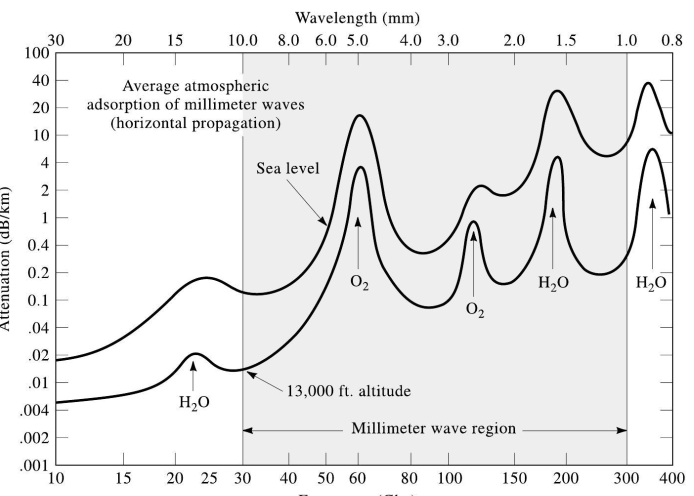
\includegraphics[width=0.75\linewidth]{Src//images/Atmospheric attenuation in the range 10-400 GHz.png}
    \caption{Atmospheric attenuation in the range 10-400 GHz\citep{fcc1997mmwave}}
    \label{fig:Atmospheric}
\end{figure}



\paragraph{24 GHz Band:} This band is often associated with lower system costs. However, it typically provides less bandwidth (around 250 MHz, though wider bandwidths up to 1 GHz or more are possible in some regions/applications) compared to higher frequency bands. This limited bandwidth restricts the achievable range resolution. Despite this, 24 GHz radars are used for applications such as presence detection and in some older or lower-cost automotive systems.

\paragraph{60 GHz Band:} The 60 GHz band offers wider bandwidths, some systems utilizing up to 7 GHz. This wider bandwidth translates to range resolution, making it applicable for short-range sensing applications where detailed environmental perception is needed. Such applications include gesture recognition, vital signs monitoring, and, increasingly. A notable characteristic of the 60 GHz band is its susceptibility to higher atmospheric absorption, primarily due to oxygen molecules. Although this can limit the maximum operational range, it also serves to reduce interference between nearby 60-GHz radar systems, which can be a feature in environments with multiple robots or sensors.

\paragraph{77-81 GHz Band (often referred to as 77 GHz or 76-81 GHz):} This frequency band has become the benchmark for automotive radar, supporting both advanced driver assistance systems (ADAS) or emergency brake system and the necessary features for autonomous vehicles. Its broad acceptance is attributed to the generous bandwidths available (starting at 4 GHz), which give a high level of accuracy in detecting and tracking objects over medium distances. 




\subsection{Candidate mmWave Radar Modules}
To select the sensor, a review of commercially available low-power radar modules frequently used in consumer electronics and IoT devices was conducted (see table \ref{tab:mmwave_sensors} and Figure \ref{fig:Radarmodels}). Data were obtained from manufacturer datasheets and marketing brochures.
% Requires: \usepackage{graphicx}% Requires: \usepackage{graphicx}
\begin{table}[h]
    \caption{Overview of Low-Cost Radar Modules}
    \label{tab:mmwave_sensors}
    \centering
    \renewcommand{\arraystretch}{1.2}
    \resizebox{\textwidth}{!}{%
    \begin{tabular}{|>{\raggedright\arraybackslash}p{3cm}|>{\raggedright\arraybackslash}p{1cm}|>{\raggedright\arraybackslash}p{3.5cm}|>{\raggedright\arraybackslash}p{1cm}|>{\raggedright\arraybackslash}p{1cm}|>{\raggedright\arraybackslash}p{3cm}|>{\raggedright\arraybackslash}p{1.5 cm}|>{\raggedright\arraybackslash}p{2.3cm}|}
        \hline
        \textbf{Model} & \textbf{Freq. (GHz)} & \textbf{Functional} & \textbf{$P_{\mathrm{TX}}$ (dBm)} & \textbf{Range (m)} & \textbf{Interface} & \textbf{Output} & \textbf{Size (mm)} \\
        \hline
        LD012-5G & 5.8 & Radar induction sensor & 3 & 0.08 & Digital & Digital & 20$\times$20$\times$3 \\
        \hline
        LD101 & 10 & Intelligent microwave radar & 2 & 0.03 & TTL & Digital & 20$\times$25$\times$4 \\
        \hline
        BGT24LTR11N16 & 24 & Presence detection & 13 & $\sim$10 & UART & — & 50$\times$35$\times$6 \\
        \hline
        HLK-LD2410C & 24 & Human body tracking & — & 6 & UART & — & 22$\times$16$\times$16 \\
        \hline
        HLK-LD2410B & 24 & Intelligent microwave radar & 13 & 6 & Serial & Serial & 35$\times$7$\times$3 \\
        \hline
        HLK-LD2461 & 24 & Human body tracking & — & 8 & — & — & 50$\times$35$\times$6 \\
        \hline
        HLK-LD2415H & 24.075 & Detection speed radar & 20 & >180 & — & — & 69$\times$53$\times$5 \\
        \hline
        BGT60LTR13C & 60 & Low-power motion detection & 10 & >10 & SPI & Digital & 64$\times$25$\times$5 \\
        \hline
        BGT60ATR24C & 60 & High-performance automotive radar & 15 & >20 & CAN & Analog/ Digital & 26$\times$16$\times$5 \\
        \hline
        IWR6843 & 60 & Smart motion detectio & 12 & >50 & SPI/ UART & — & 154$\times$152$\times$18 \\
        \hline
        IWR1443 & 76–81 & Automotive radar for ADAS & 15 & >100 & SPI/CAN & — & 154$\times$152$\times$18 \\
        \hline
        IWR1843 & 76–81 & High-resolution radar & 18 & >150 & SPI/CAN & Digital & 154$\times$152$\times$18 \\
        \hline
    \end{tabular}%
    }
   
\end{table}
\noindent
\textbf{Sensor Analysis}

\begin{figure}
    \centering
    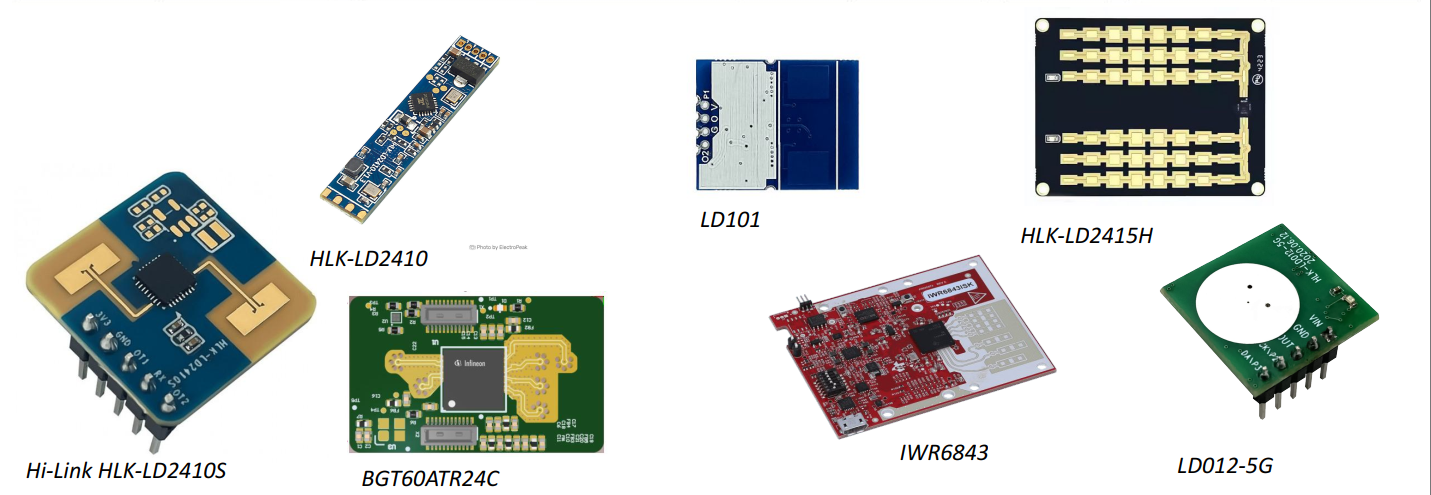
\includegraphics[width=0.8\linewidth]{Src/images/Radarmodels.png}
    \caption{Radar models}
    \label{fig:Radarmodels}
\end{figure}
\begin{itemize}
\item \textbf{5.8–10\;GHz (LD012-5G, LD101).} These sensors are extremely compact and inexpensive, but their range is limited to just a few centimeters. They are only suitable for simple presence detection and are entirely inadequate for navigation tasks.
  
\item \textbf{24\;GHz family (BGT24LTR11N16, HLK-LD24xx).} Widely used in smart home systems. Their effective range of 6–10 m makes them suitable for corridors and small rooms. However, the larger antenna size and lower angular resolution compared to 60\;GHz units limit their spatial performance. The lack of integrated MIMO arrays further complicates direction-of-arrival (DoA) estimation.

\item \textbf{60\;GHz low-power (BGT60LTR13C).} Offers an optimal trade-off between size, power, and capability. The compact antenna-in-package design and power consumption below 100 mW make it ideal for mobile use. Range exceeds 10 m, and raw FMCW data is available over SPI. 

\item \textbf{60\;GHz high-end (BGT60ATR24C, IWR6843).} Equipped with enhanced MIMO configurations and onboard DSP, these sensors support range up to 50 m and angular localization. However, their size and cost are higher, which may be excessive for small indoor environments.

\item \textbf{76–81\;GHz automotive-grade (IWR1443/1843).} Designed for ADAS applications, these units offer superior resolution and range exceeding 100 m. However, they consume significantly more power and require complex circuitry. They are excluded from consideration due to the thesis focus on low-cost and low-power platforms.
\end{itemize}

\noindent
\noindent
\noindent
Consequently, was taken low-power 60 GHz radars (BGT60LTR13C Figure \ref{fig:BGT60TR13C}), offer the compromise between size, cost, and power consumption. Sensors are primarily designed for detecting human presence, gestures, or analysing micro-movements such as breathing and heartbeat.
\begin{figure}[H]
    \centering
    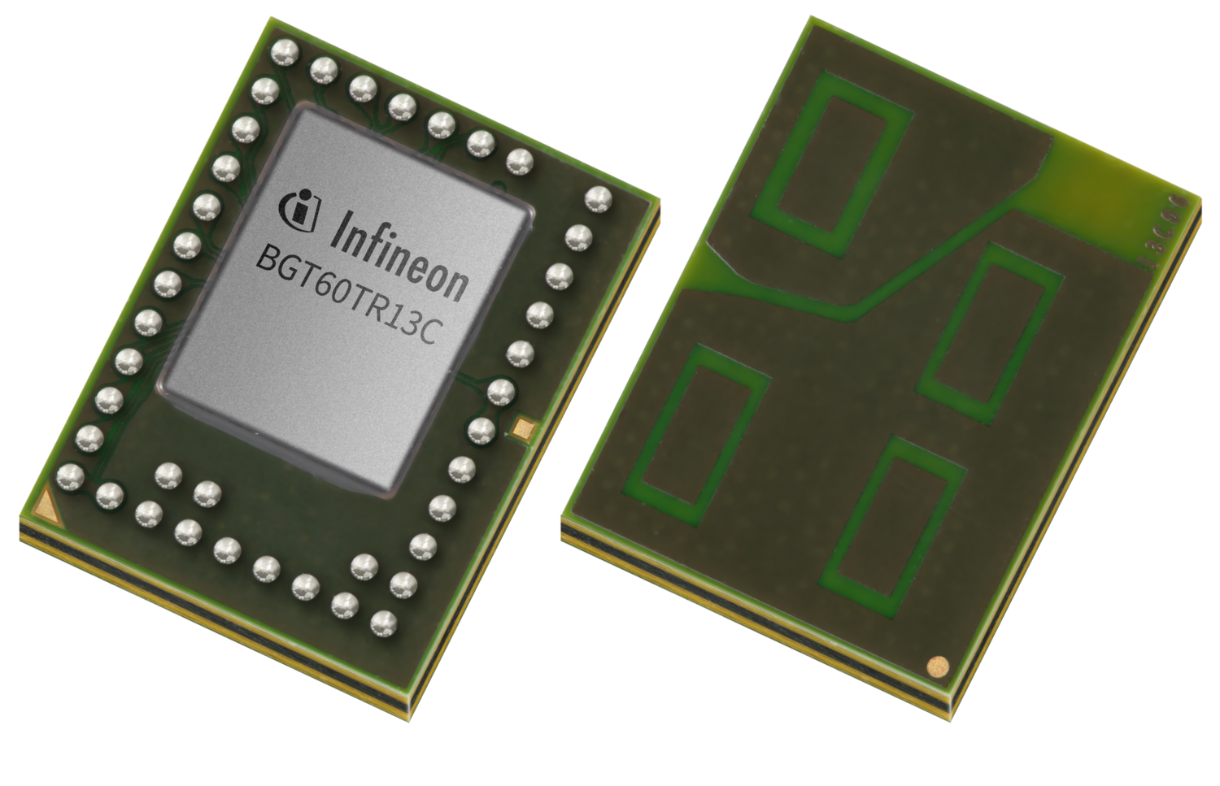
\includegraphics[width=0.5\linewidth]{Src/images/lowres-BGT60_WFWLB-40_Combi.tif.png_620533323.png}
    \caption{BGT60TR13C SoC}
    \label{fig:BGT60TR13C}
\end{figure}
An important advantage of the chip is that the BGT60LTR13C is a complete radar-on-chip (SoC) solution: it integrates both the RF front end and the antenna array in a single package using AiP (antenna-in-package) technology. There is no need to develop an external RF circuit or place antennas. As a result, no printed circuit board or high-frequency substrate is required.
\begin{table}[h]
\centering
\caption{Characteristics of the Infineon BGT60TR13C 60 GHz Radar Sensor}
\label{tab:bgt60tr13c_specs}
\begin{tabular}{p{4.5cm} p{8cm}}
\toprule
\textbf{Characteristic} & \textbf{Description} \\
\midrule
\textbf{Operating Frequency} & 57--64 GHz (FMCW) \\
\textbf{Bandwidth} & 5.5 GHz, enabling $\sim$3 cm range resolution \\
\textbf{Antenna Configuration} & 1 Tx, 3 Rx (L-shaped array for horizontal and vertical angular measurement) \\
\textbf{Field of View (FoV)} & Azimuth:$-45^\circ$ to$+45^\circ$, Elevation:$-45^\circ$to$+45^\circ$ \\
\textbf{Power Supply} & 1.8 V (optional 3.3 V for loop filters) \\
\textbf{Power Consumption} & less than 5 mW \\
\textbf{Current Consumption} & 200 mA at 1.8 V  \\
\textbf{Package Size} & 6.5 $\times$ 5.0 $\times$ 0.9 mm$^3$ (Antennas in Package) \\
\textbf{Interface} & Serial Peripheral Interface (SPI) for configuration and data acquisition  \\
\textbf{Chirp Ramp-Up Speed} & 400 MHz/$\mu$s, supporting high Doppler velocity  \\
\textbf{Detection Range} & Up to 10 m (front-facing human detection) \\
\textbf{Sensitivity} & Detects sub-millimeter movements (vital signs) \\
\textbf{Integrated Features} & Finite-State Machine (FSM) for autonomous FMCW chirps and data storage \\
\textbf{Applications} & Presence detection, gesture sensing, vital sign monitoring, material classification\\
\bottomrule
\end{tabular}
\end{table}



Infineon offers several models in its 60 GHz radar sensor family, each tailored to specific applications \citep{Infineon2022BGT60TR13C}. For example, the BGT60LTR11, a simpler model, features a single transmit antenna (Tx) and receive antenna (Rx), lacking spatial diversity and therefore unable to determine the direction of incoming signals \citep{Infineon2021BGT60LTR11}. 

\begin{figure}[H]
    \centering
    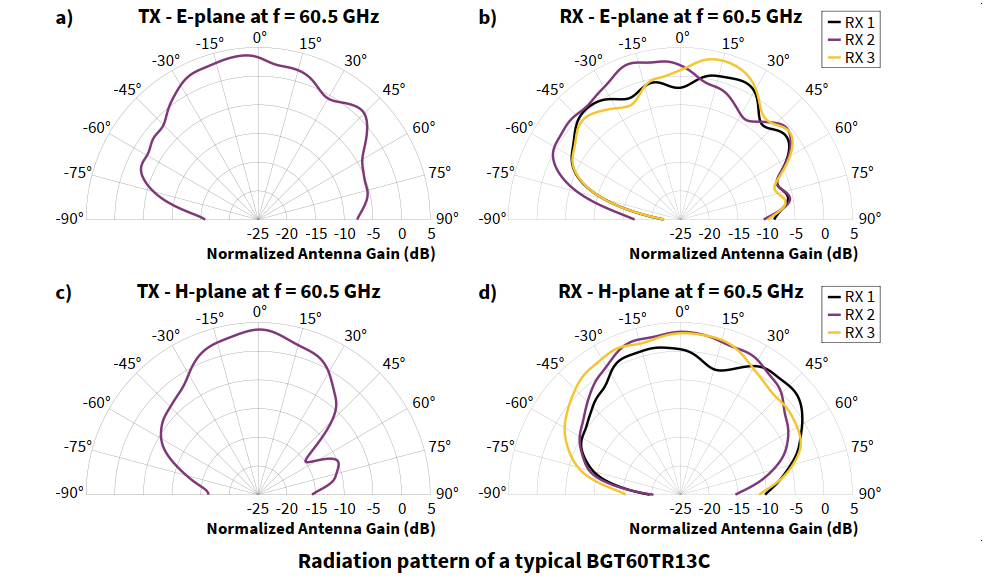
\includegraphics[width=0.9\linewidth]{Src/images/radarpattern.png}
    \caption{Radiation pattern of a typical BGT60TR13C  \citep{infineon_bgt60tr13c}}
    \label{fig:radar-patern}
\end{figure}


While using only two antennas limits the ability to exploit the features of an antenna array, the radar module overcomes this by integrating three receive antennas in an L-shaped configuration, enabling the estimation of both azimuth and elevation angles \citep{Infineon2022BGT60TR13C, Wevolver2023BGT60TR13C}.

The technical description of the radar module \citep{Infineon2022BGT60TR13C} contains only limited information about the antenna characteristics, specifically listing the beam width at \textbf{3 dB} for the transmit and receive channels. The real antenna radiation pattern is characterized along two main planes \ref{fig:radar-patern}: the \textbf{E-plane} and the \textbf{H-plane}, representing the vertical and horizontal field orientations, respectively. The image shows measured antenna gain patterns at an operating frequency of \textbf{60.5 GHz}.

In the \textbf{E-plane} (Figures \textbf{a} and \textbf{b}), both the transmit and receive antennas show pronounced side lobes and a main lobe shifted approximately \textbf{ 25 \degree } from the normal to the board surface. This angular offset is caused by near-field coupling effects due to the compact placement of antenna elements and is more pronounced for electric fields.
In the \textbf{H-plane} (Figures \red{fig:radar-patern} c and d), the radiation patterns are more symmetric: the main lobe points perpendicular to the chip surface and the side lobes are not present, making this plane preferable for vertical detection.



% \subsection{ROS2}
% Все программные компоненты реализованы поверх \textbf{ROS2 Humble Hawksbill}.

% \begin{enumerate}
% \item \textbf{Драйвер радара} (\texttt{mmwave\_driver}): C++ rclcpp node, который конфигурирует BGT60TR13C по SPI и публикует два топика: сырой ADC-фрейм и облако точек после onboard-DSP.
% \item \textbf{Трекер целей} (\texttt{radar\_tracker}): реализует фильтр Калмана в пространстве \$x\$–\$y\$–\$v\_r\$, ассоциирует точки между кадрами и присваивает ID объектам.
% \item \textbf{Интеграция с Nav2}: кастомный плагин \texttt{RadarLayer} добавляет в локальную costmap динамические препятствия с временным затуханием 0,5 с.
% \item \textbf{Симуляция}: плагин mWaveRadarSensor для Gazebo Fortress с использованием RTTI модели распространения; обеспечивается идентичность формата данных между симуляцией и аппаратными испытаниями.
% \item \textbf{CI/CD}: сборка пакетов через \texttt{colcon}; GitHub Actions проверяют компиляцию на x86 и ARM, а также выполняют модульные тесты Google CTest.
% \end{enumerate}

% %----------------------------------------------------


% \subsection{Features of radar signals}

% % Сырой сигнал FMCW-радара проходит сложную цепочку обработки, прежде чем превратиться в понятные роботам сведения об окружающей среде. Низкоуровневая обработка (DSP): на борту радара выполняется микширование отражённого сигнала с эталонным, оцифровка и вычисление диапазонной FFT для получения спектра отражений по дальности Этот спектр часто оформляется как range-Doppler матрица – двумерное представление, где одна ось – дальность, другая – доплеровская скорость. Далее применяется алгоритм CFAR (Constant False Alarm Rate) – адаптивная пороговая фильтрация, выделяющая пики над шумом на спектральной матрице Смысл CFAR в том, чтобы автоматически подстраивать порог детектирования под уровень шума в локальном окне спектра, обеспечивая фиксированную вероятность ложной тревоги. Различают несколько видов CFAR (с усреднением по окружению, порядковой статистикой и др.), но суть одна: сравнивать каждый резонансный сигнал с локальным фоном и отсекать шумовые всплески


% % \subsubsection{FMCW features in radar systems}
% % \subsubsection{Pulse compression}
% % \subsubsection{Frequency modulation}
% % \subsubsection{Pulse repetition frequency}
% % \subsubsection{Bandwidth}
% % \subsubsection{Resolution}
% % \subsubsection{Range}


% \subsection{Radar connection diagram}


% \subsection{Comparison of Radar System Parameters}

